% !TeX root = Protokoll.tex
\begin{figure}[h!]
\centering
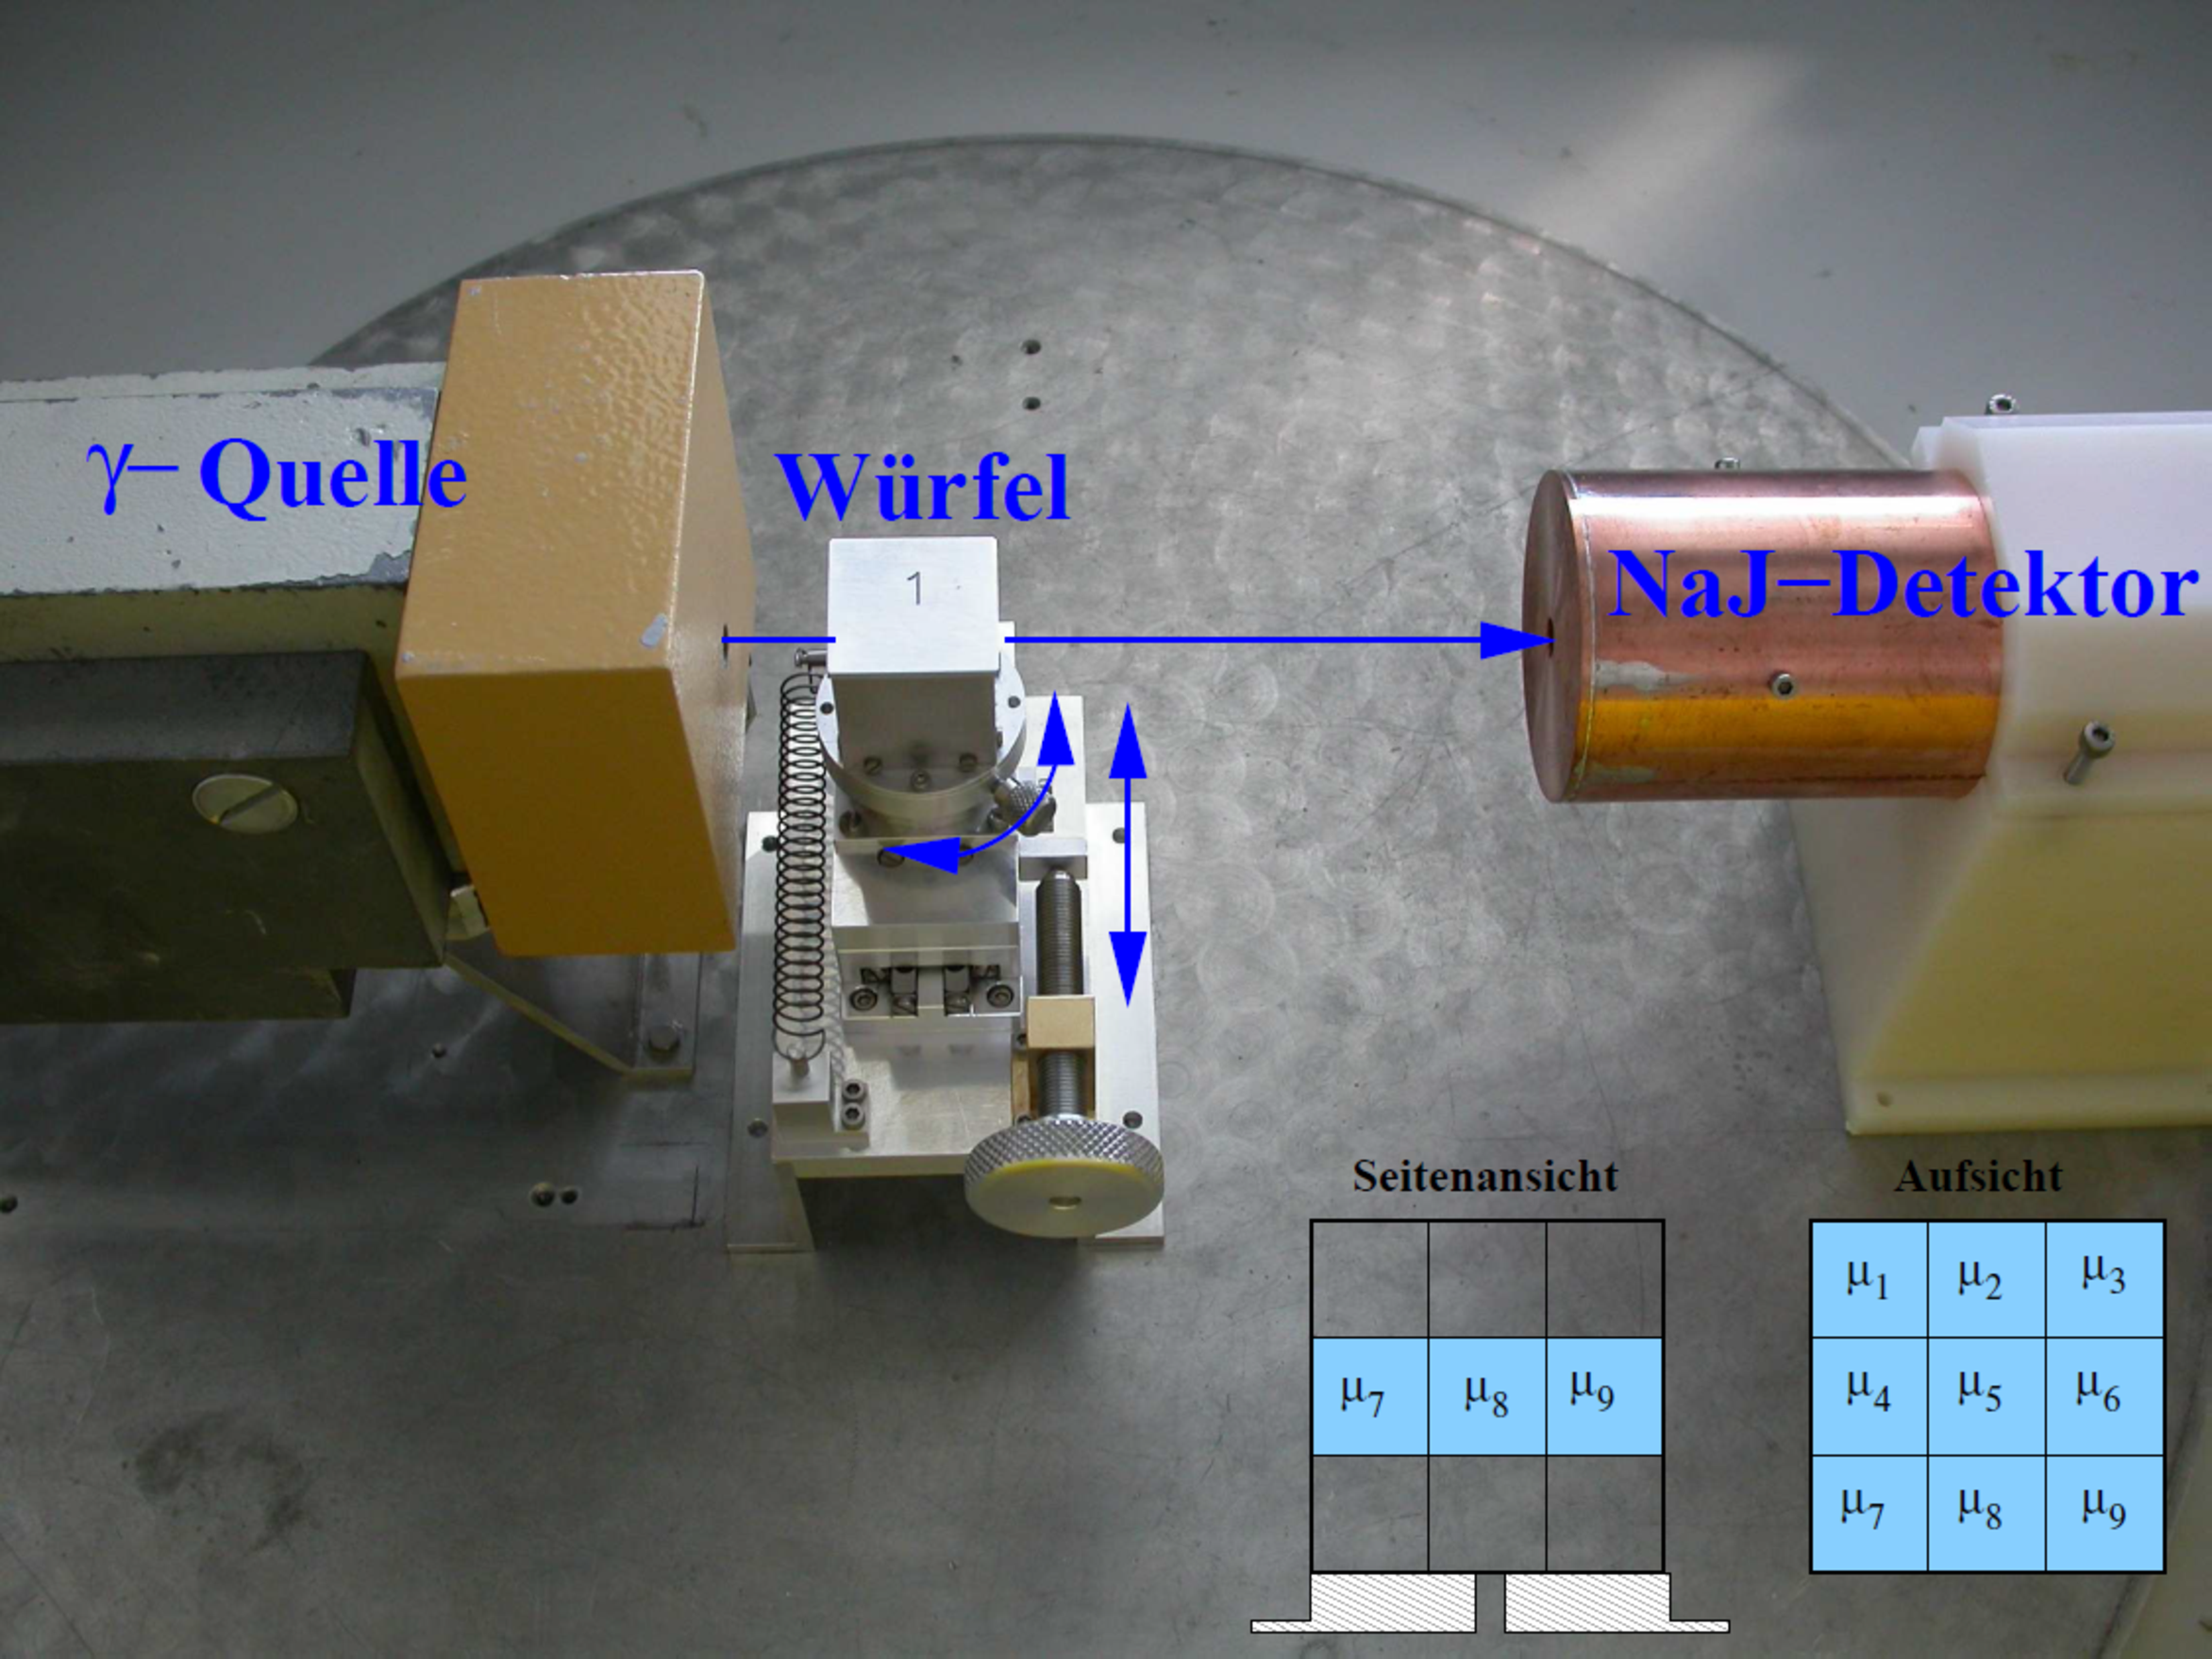
\includegraphics[width = 0.75\textwidth]{../Grafiken/Aufbau.pdf}
\caption{Die Darstellung des Verwendeten Aufbaus \cite{V14}.}\label{fig:Aufbau}
\end{figure}
In \cref{fig:Aufbau} ist der Aufbau dargestellt.
Die Quelle die in diesem Versuch für die $\gamma$-Strahlung verwendet wird, ist ${}^{137}_{55}$Cs.
Diese Zerfällt unter Ausstrahlung von $\beta$-Strahlung in ein ${}^{137m}_{56}$Ba.
Dies zerfällt durch Abstrahlung von $\gamma$-Strahlung in ${}^{137}_{56}$Ba.
Die $\gamma$-Strahlung besitzt dabei eine Energie von $E_\gamma$=0,6617MeV.
%Zerfällt durch den Zerfall in den nicht angeregten Zustand wird $\gamma$-Strahlung emittiert mit der Energie $E_\gamma$=0,6617MeV. Ein Schema ist in \cref{fig:Energieschema} dargestellt.
\\
Als erstes wird ein Würfel vermessen, dessen Inhalt Luft ist, dadurch lässt sich die Auswirkung der Ummantelung der Würfel heraus rechnen, sowie Untergrund, der durch die Umgebung entsteht.
Danach werden die Würfel mit der Kennung 1 und 2 vermessen, deren Elementarwürfel aus einem Stoff bestehen.
Zum Schluss wird der Würfel mit der Kennung 3 vermessen, die Zusammensetzung der Elementarwürfel ist hier unbekannt. 
Die Würfel werden nach einander in der Strahlengang gestellt und nach \cref{fig:Projektion} bestrahlt.
Dabei müssen die Anzahl der Projektionen größer sein, als die Anzahl der Elementarwürfel, damit eine genauere Vermessung möglich ist.\\
Dabei wurde für jeden Würfel die eine Bestrahlungsdauer gewählt, so dass bei der ersten diagonalen Bestrahlung ($I_2$) ein Fehler weniger als $3\%$ auftritt.
%Die Strahlung wechselwirkt mit dem Material, überwiegend durch den Compton- und über den Photo-Effekt.\\
Die Strahlung wird mithilfe eines Szintillationsdetektors nachgewiesen.
In dem Detektor werden durch die einfallende Strahlung Photonen ausgelöst, deren Anzahl proportional zur Energie der einfallenden Strahlung ist.
Die Ereignisse werden mithilfe eines Diskriminators und eines Multichannelanalyzers in Kanälen gespeichert, die proportional zur Energie sind.
Die Daten werden mithilfe eines PC ausgelesen.
\begin{figure}[h!]
	\centering
	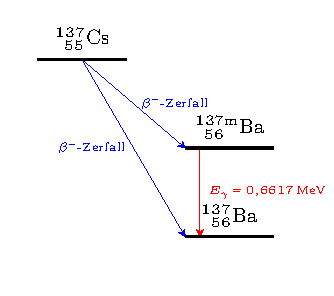
\includegraphics[width = 0.5\textwidth]{../Grafiken/Tikz/tikz-Energieschema.pdf}
	\caption{Eine Schematische Darstellung des Zerfalls der ${}^{137}_{\,\,\, 55}$Cs Quelle.}\label{fig:Energieschema}
\end{figure}